% Tipo de documento
\documentclass[11pt,a4paper]{article}

% Pacotes
%\usepackage{showlabels}
\usepackage{latexsym}
\usepackage{amsfonts}
\usepackage{amsmath}
\usepackage{amscd}
\usepackage[brazil]{babel}
\usepackage[utf8]{inputenc}
\usepackage[pdftex]{graphicx} 

% Paginação
\textwidth 16.5cm                     % Largura
\textheight 24.5cm                    % Altura
\addtolength{\oddsidemargin}{-2.0cm}  % Margem esquerda (impar)
\addtolength{\topmargin}{-2.0cm}      % Margem superior

% Estilo dos parágrafos
\sloppy                              % Mais flexível
\setlength{\jot}{08pt}               % Distância entre linhas do eqnarray
\setlength{\parskip}{1ex}            % Distância entre parágrafos
\renewcommand{\baselinestretch}{1.0} % Distância entre linhas

% Contagem de equações por seção
\renewcommand{\theequation}{\thesection.\arabic{equation}}

% Contagem de figuras por seção
\renewcommand{\thefigure}{\thesection.\arabic{figure}}

% Contagem de tabelas por seção
\renewcommand{\thetable}{\thesection.\arabic{table}}

% Zerar as contagem em cada seção
\newcommand{\zerar}{\setcounter{equation}{0}\setcounter{figure}{0}\setcounter{table}{0}}

\DeclareMathOperator{\col}{col}
\DeclareMathOperator{\row}{row}

% Conjunto de números
\newcommand{\Z}{\mathbb{Z}}
\newcommand{\C}{\mathbb{C}}
\newcommand{\N}{\mathbb{N}}
\newcommand{\Q}{\mathbb{Q}}
\newcommand{\R}{\mathbb{R}}

%%%%%%%%%%%%%%%%%%%%%%%%%%%%%%%%%%%%%%%%%%%%%%%%%%%%%%%%%%%%%%%%%%%%%%%%%%%%%%%%%%%%%%%%%%%%%%%%%%%%

\begin{document}

\title{
  {\sc MAC0438 -- Programação Concorrente} \\ 
  \vspace{0.5cm} 
  {\bf Jantar dos Selvagens}
}
\author{Daniel Augusto Cortez -- 2960291}
%\date{12 de junho de 2014}
\date{}
\maketitle

%%%%%%%%%%%%%%%%%%%%%%%%%%%%%%%%%%%%%%%%%%%%%%%%%%%%%%%%%%%%%%%%%%%%%%%%%%%%%%%%%%%%%%%%%%%%%%%%%%%%

\zerar
\section{Introdução}
\label{sec:intro}

Este relatório descreve a implementação proposta para resolver o problema do jantar dos selvagens, 
bem como apresenta os resultados dos experimentos sugeridos para análise das soluções obtidas. 

A localização do código-fonte com as funções exigidas para manipulação do monitor e a forma de 
utilização do programa estão disponíveis no arquivo \verb|README|.

%%%%%%%%%%%%%%%%%%%%%%%%%%%%%%%%%%%%%%%%%%%%%%%%%%%%%%%%%%%%%%%%%%%%%%%%%%%%%%%%%%%%%%%%%%%%%%%%%%%%

\zerar
\section{Implementação}
\label{sec:imp}

A implementação foi escrita em Java (1.7.45) no ambiente de desenvolvimento Eclipse (Kepler). O 
arquivo \verb|DiningSavages.jar| deve ser utilizado para executar o programa.

O monitor implementado na classe \verb|PotMonitor.java| garante o acesso exclusivo ao pote pelos
selvagens e pelos cozinheiros. Em alto nível, sem se preocupar com detalhes como o número de vezes 
que o pote é esvaziado (repetições) e as informações a serem impressas, o código do monitor pode ser 
escrito como abaixo:

\begin{verbatim}
  monitor Pot {
    int portions = C;
    cond potEmpty, potFull;

    procedure eatPortion(Savage savage) {
      while (portions == 0) {
        # O primeiro faminto que percebe o pote vazio acorda um cozinheiro
        if (empty(potFull)) signal(potEmpty);
        wait(potFull);  # wait(potFull, rank(savage)) 
      }
      portions = portions - 1;
    }

    procedure makePortions(Cook cook) {
      while (portions > 0) wait(potEmpty);
      portions = C;
      signal_all(potFull);
    }
  }
\end{verbatim}

Foram utilizadas duas variáveis de condição: \verb|potEmpty| para indicar quando o pote está vazio, 
e \verb|potFull| para indicar quando o pote está cheio. O contador \verb|portions| conta quantas 
porções estão disponíveis no pote. Se \verb|portions = 0| o pote está vazio. Se 
\verb|portions = C| o pote está cheio. A constante $C$ é a capacidade do pote informada no arquivo 
de entrada. Note que apenas o primeiro faminto que observa o pote vazio ao tentar comer dele é o 
responsável por acordar um cozinheiro. Note também que se um cozinheiro tiver acesso ao monitor e 
verificar que o pote está vazio, ele completará o pote com novas porções. 

O \verb|wait| com prioridade foi utilizado no caso em que a simulação roda com pesos. Nesse caso, 
selvagens mais gordos são colocados primeiro na fila da variável \verb|potFull|. Quando essa 
condição é verdadeira, eles acessam primeiro o pote, e portanto, podem comer mais.

Pela necessidade de se implementar um monitor com prioridades, não se utilizou o métodos padrões
\verb|wait()| e \verb|notify()| do Java. A implementação do monitor foi feita com base em semáforos,
conforme exposto nos slides da Aula~18. Um {\it lock} é utilizado dentro do  monitor para garantir o
acesso exclusivo aos métodos. Cada variável de condição possue um vetor  privado de semáforos e uma
fila de threads. Cada thread na fila aguarda em um semáforo específico do  vetor. A implementação da
variável de condição é feita na classe \verb|CondionVariable.java|. Note  que na implementação
utilzou-se uma lista ligada para a fila de threads e um \verb|HashMap| para o vetor de semáforos.
Quando se deseja colocar uma thread na fila com prioridade, essa thread deve  implementar a
interface \verb|Rankable|. Com isso, pode-se extrair o valor do {\it rank} associado à thread e
inserí-la em ordem na fila.

O selvagem é implementado na classe \verb|Savage.java|. Ela estende a classe \verb|Thread|. O seu 
método \verb|run()| chama o procedimento \verb|eatPortion()| do monitor enquanto o número de 
repetições do pote não se esgotar.

O cozinheiro é implementado na classe \verb|Cook.java|. Ela estende a classe \verb|Thread|. O seu 
método \verb|run()| chama o procedimento \verb|makePortions()| do monitor enquanto o número de 
repetições do pote não se esgotar.

A classe \verb|DinigSavages.java| contém o método \verb|main()| do programa. Ele efetua a leitura
dos parâmetros e faz a instanciação dos objetos de acordo (selvagens, cozinheiros e o monitor). 
Em seguida, inicializa as threads rodando a simulação.

O número de repetições, que equivale ao número de vezes que o pote é esvaziado, é controlado
pelo monitor. Esse número é lido da linha de comando e passado ao monitor em sua instancialização.
Toda vez que o pote é esvaziado por algum selvagem, o número de repetições é decrementado. Quando
esse contador atinge o valor zero, todos as threads são sinalizadas. Ao acordar, a primeira coisa
que uma thread faz é verificar se o número de repetições é positivo. Caso negativo, o {\it lock} é
liberado e ela imediatamente sai do procedimento. Os procedimentos dos selvagens e cozinheiros são
iterados enquanto o número de repetições for positivo.

%%%%%%%%%%%%%%%%%%%%%%%%%%%%%%%%%%%%%%%%%%%%%%%%%%%%%%%%%%%%%%%%%%%%%%%%%%%%%%%%%%%%%%%%%%%%%%%%%%%%

\section{Experimentos}
\label{sec:exp}

Algumas simulações forma realizadas para testar o correto funcionamento do programa. Elas foram 
executadas em uma máquina com processador Intel Core i5 (1.6 GHz) com 4Gb de memória RAM, rodando o 
sistema operacional MacOS~10.9.2.

Foram utilizados dois arquivos de entrada: \verb|simples.txt| e \verb|complexo.txt|. O primeiro 
arquivo representa um cenário simples com 6~selvagens e 3~cozinheiros. O segundo arquivo representa 
um cenário complexo com 20~selvagens e 10~cozinheiros. Os números foram escolhidos de forma 
arbitrária. A capacidade do pote utilizada no caso simples foi $C = 2$ e no caso complexo $C = 12$. 
Cada cenário foi avaliado nos casos uniforme e com pesos através de 1000 repetições. Os dados 
resultantes dos testes estão disponíveis no arquivo \verb|experimentos.xlsx|.

A Figura~\ref{fig:us} apresenta os resultados da simulação do cenário simples no caso uniforme. Do
lado esquerda apresenta-se um gráfico (Gráfico~1 do enunciado do EP) em que o eixo horizontal
representa o tempo lógico da simulação (número de vezes que o pote foi enchido), e o eixo vertical
representa o  número médio de vezes que cada cozinheiro acordou. Do lado direito apresenta-se um
gráfico (Gráfico~2 do enunciado do EP) em que o eixo horizontal representa os selvagens, e o eixo
vertical representa o número de porções que cada selvagem comeu.

A Figura~\ref{fig:ps} apresenta os resultados da simulação do cenário simples no caso com pesos. A 
descrição dos gráficos apresentados é a mesma que no caso anterior.

\begin{figure}[htbp]
  \begin{center} 
    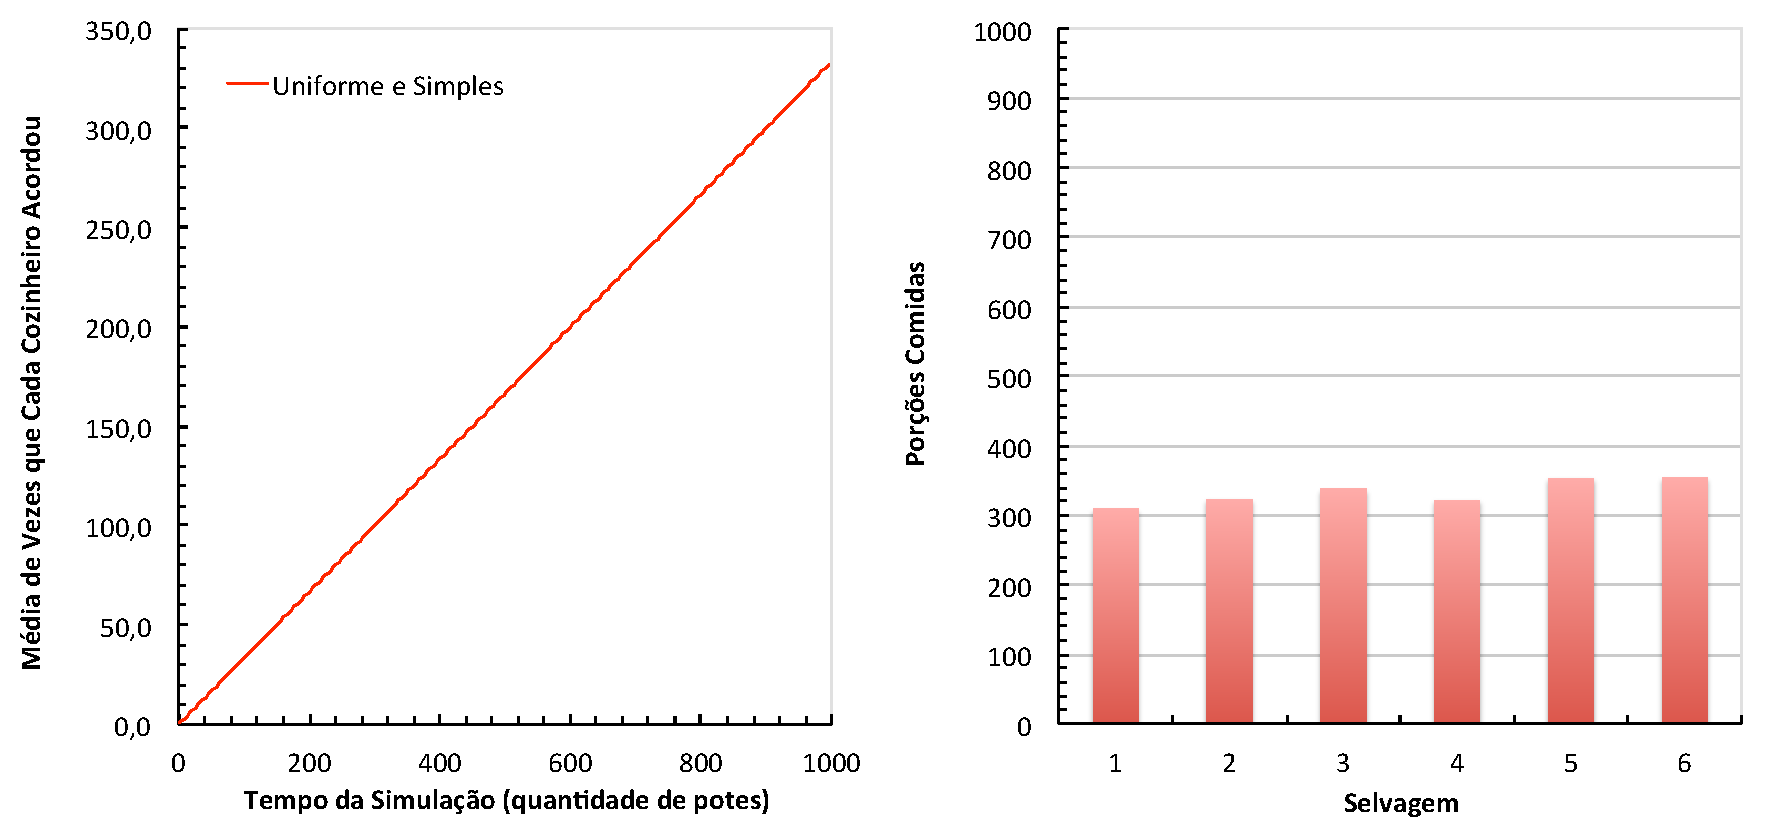
\includegraphics[scale=0.5]{uniforme_simples.pdf}
    \caption{Gráficos 1 e 2 para o cenário simples no caso uniforme.}
    \label{fig:us}
  \end{center}
\end{figure}
%
\begin{figure}[htbp]
  \begin{center}
    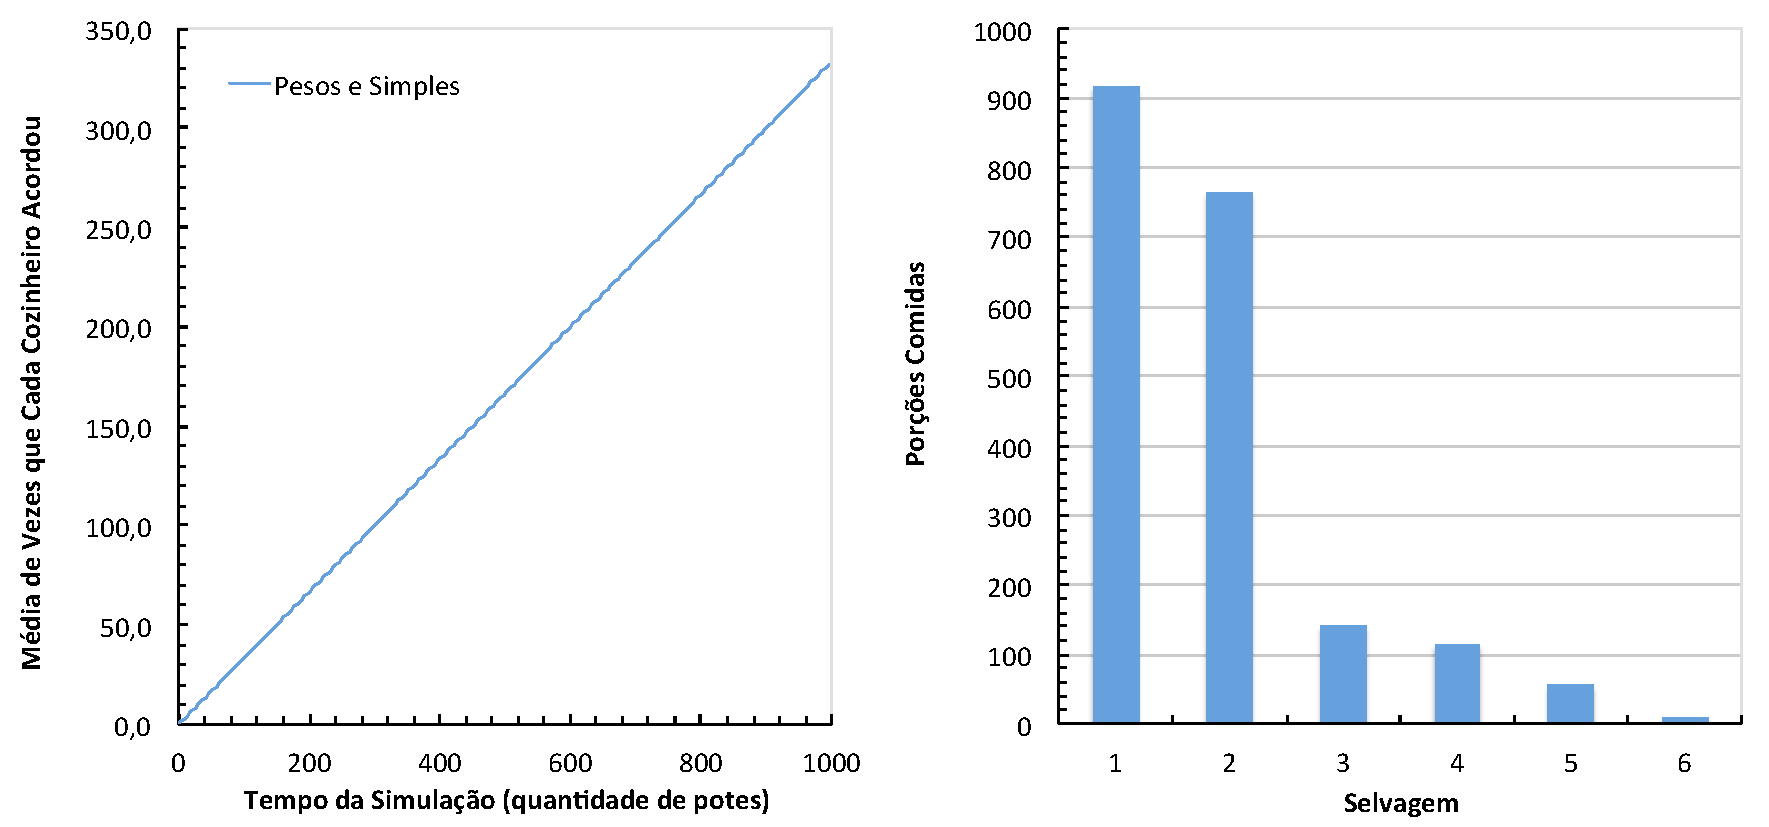
\includegraphics[scale=0.5]{pesos_simples.pdf}
    \caption{Gráficos 1 e 2 para o cenário simples no caso com pesos. Os pesos atribuídos aos 
    selvagens foram 6, 5, 4, 3, 2, 1.}
    \label{fig:ps}
  \end{center}
\end{figure}

As Figura~\ref{fig:uc} e~\ref{fig:pc} apresentam os resultados da simulação do cenário complexo nos 
casos uniforme e com pesos, respectivamente. A descrição dos gráficos apresentados é a mesma que nos 
casos anterioriores.

\begin{figure}[htbp]
  \begin{center} 
    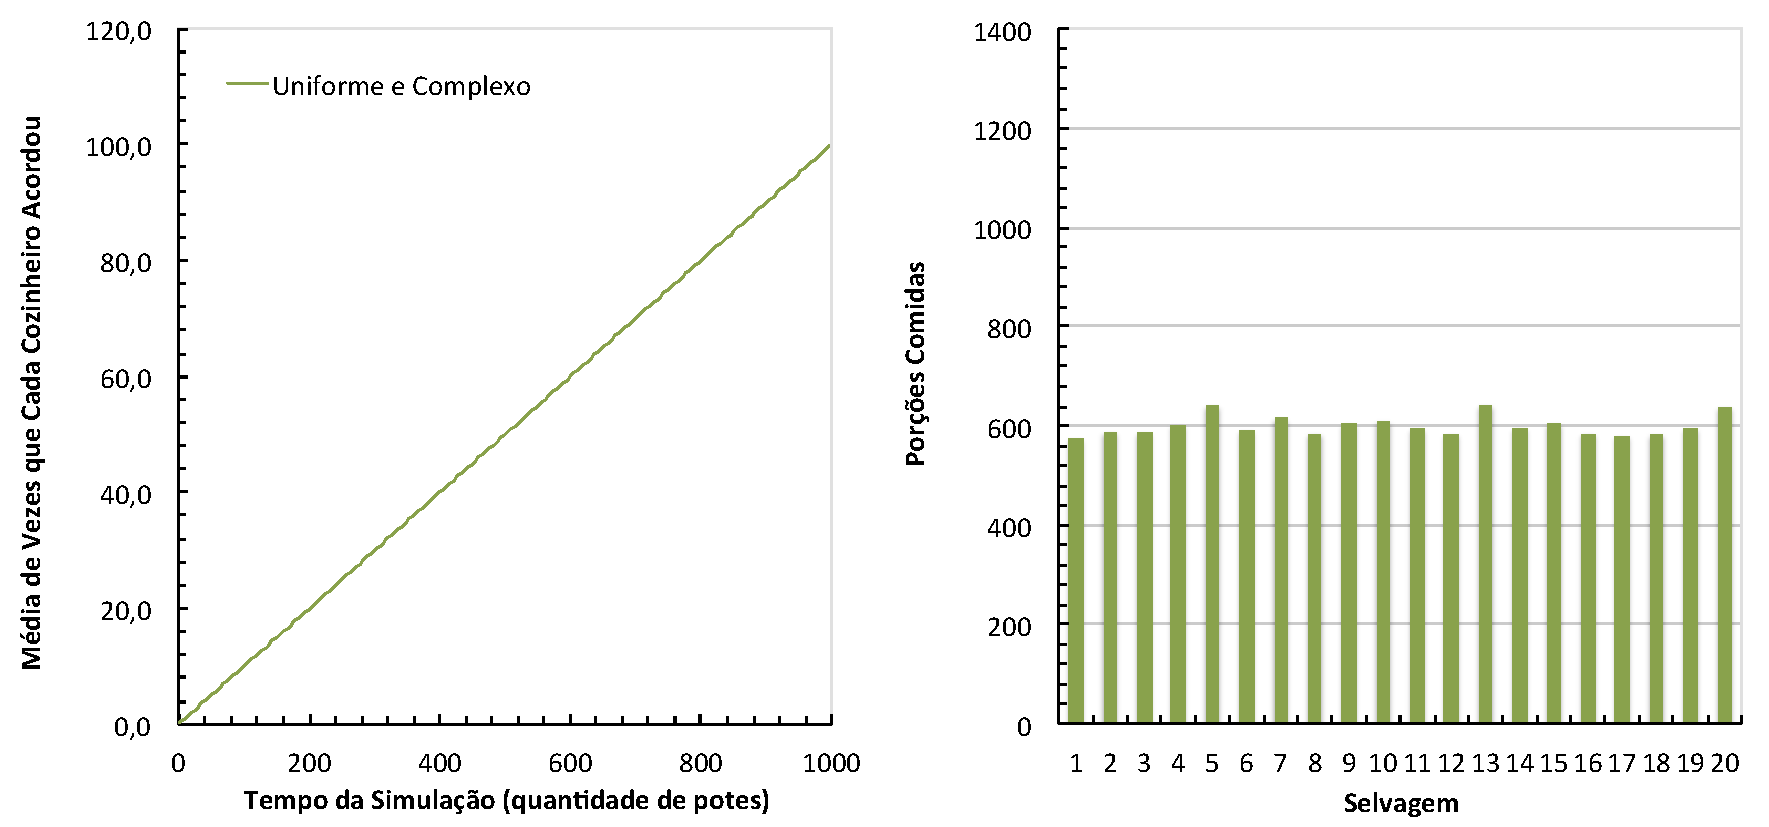
\includegraphics[scale=0.5]{uniforme_complexo.pdf}
    \caption{Gráficos 1 e 2 para o cenário complexo no caso uniforme.}
    \label{fig:uc}
  \end{center}
\end{figure}
%
\begin{figure}[htbp]
  \begin{center} 
    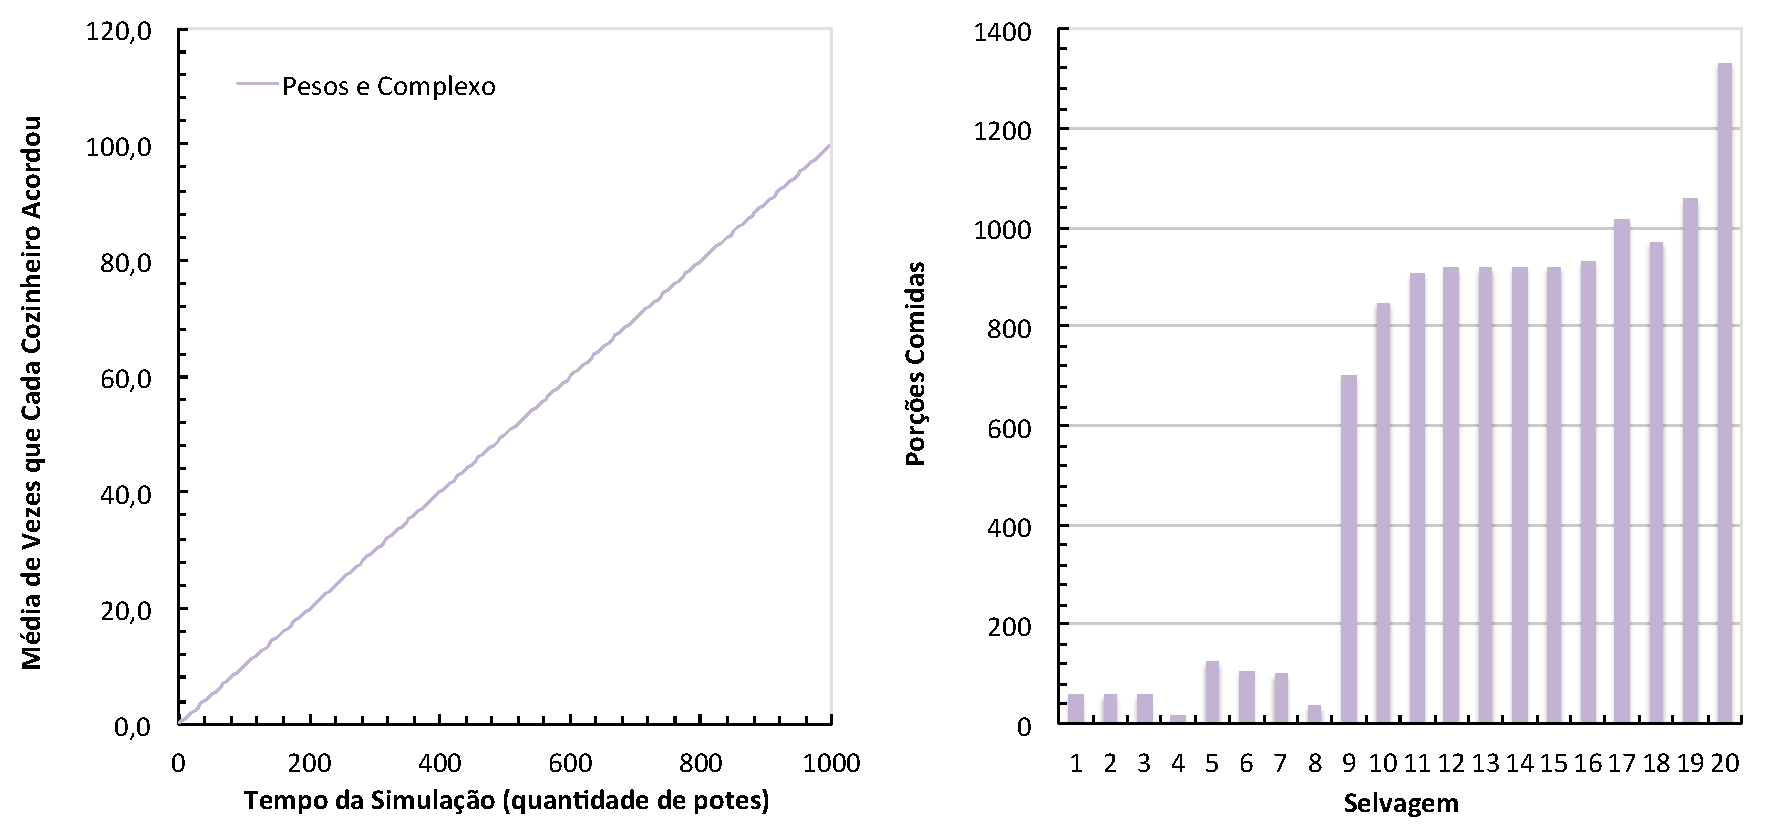
\includegraphics[scale=0.5]{pesos_complexo.pdf}
    \caption{Gráficos 1 e 2 para o cenário complexo no caso com pesos. Os pesos atribuídos aos 
    selvagens foram 1, 2, 3, 4, 5, 6, 7, 8, 9, 10, 11, 12, 13, 14 15, 16, 17, 18 19, 20.}
    \label{fig:pc}
  \end{center}
\end{figure}

%%%%%%%%%%%%%%%%%%%%%%%%%%%%%%%%%%%%%%%%%%%%%%%%%%%%%%%%%%%%%%%%%%%%%%%%%%%%%%%%%%%%%%%%%%%%%%%%%%%%

\section{Conclusões}
\label{sec:conc}

O comportamento linear do gráfico~1 encontrado em todos os casos foi o esperado, indicando que os 
mecanismos de sincronização funcionaram corretamente. De fato, se a quantidade de potes é $Q$, então 
a soma de vezes que cada cozinheiro encheu o pote é $Q$, de forma que a média do número de vezes que 
cada cozinheiro acordou é $Q/M$ ($M$ é o número de cozinheiros). Isso explica as retas obtidas com 
coeficiente angular $1/6$ no cenário simples (Figuras~\ref{fig:us} e~\ref{fig:ps}, $M = 6$), e as 
retas obtidas com coeficiente angular $1/20$ no cenário complexo (Figuras~\ref{fig:uc} 
e~\ref{fig:pc}, $M = 20$).

O comportamento do gráfico~2 em todos os casos também foi o esperado. Observe como nos casos 
uniforme (Figuras~\ref{fig:us} e~\ref{fig:uc}) a quantidade de vezes que cada selvagem comeu é 
praticamente a mesma, uma vez que as barras verticais são quase do mesmo tamanho. Já no caso com 
pesos (Figuras~\ref{fig:ps} e~\ref{fig:pc}), as barras ficaram mais ou menos proporcionais aos pesos 
dos selvagens, indicando que selvagens mais gordos comeram mais do que selvagens mais magros. Isso 
indica que o mecanismo de inserir os selvagens na fila da variável de condição \verb|potFull| com 
prioridade funcionou corretamente.

Nas simulações escolhemos valores de $C$ (a capacidade do pote) que melhor ilustrassem os 
comportamentos esperados. Entretanto, observou-se que o comportamento é relativamente sensível a 
escolha desse parâmetro, sem entretanto, afetar o seu caráter qualitativo esperado.

Para finalizar, gostaríamos de destacar que a saída do programa está de acordo com a lógica 
implementada. Em particular, observa-se que sempre primeiro um selvagem nota o pote vazio, depois
é feita a impressão dos totais solicitados no enunciado, e por fim o cozinheiro acordado enche o 
pote. A saída típica é como no trecho abaixo, extraído durante a simulação do cenário simples no 
caso uniforme:

\begin{verbatim}
  ...
  (Selvagem S3 notou o pote vazio)
  Selvagem S1 comeu 126 vezes
  Selvagem S2 comeu 141 vezes
  Selvagem S3 comeu 145 vezes
  Selvagem S4 comeu 184 vezes
  Selvagem S5 comeu 121 vezes
  Selvagem S6 comeu 215 vezes
  Cozinheiro C1 encheu 156 vezes
  Cozinheiro C2 encheu 155 vezes
  Cozinheiro C3 encheu 155 vezes
  [Cozinheiro C2 encheu o pote]
  (Selvagem S3 notou o pote vazio)
  Selvagem S1 comeu 126 vezes
  Selvagem S2 comeu 141 vezes
  Selvagem S3 comeu 147 vezes
  Selvagem S4 comeu 184 vezes
  Selvagem S5 comeu 121 vezes
  Selvagem S6 comeu 215 vezes
  Cozinheiro C1 encheu 156 vezes
  Cozinheiro C2 encheu 156 vezes
  Cozinheiro C3 encheu 155 vezes
  [Cozinheiro C3 encheu o pote]
  ...
\end{verbatim}

%%%%%%%%%%%%%%%%%%%%%%%%%%%%%%%%%%%%%%%%%%%%%%%%%%%%%%%%%%%%%%%%%%%%%%%%%%%%%%%%%%%%%%%%%%%%%%%%%%%%

%\begin{thebibliography}{99}
%  \bibitem{aima} S.~Russell, P.~Norvig. {\it Artificial Intelligence -- A Modern Approach}. Segunda
%  edição.
%\end{thebibliography}

\end{document}
